\documentclass[14pt, a4paper]{article}
\usepackage[14pt]{extsizes} % для того чтобы задать нестандартный 14-ый размер шрифта
\usepackage[utf8]{inputenc}
\usepackage{cmap}

\RequirePackage{caption}
\DeclareCaptionLabelSeparator{defffis}{ -- }
\captionsetup{justification=centering,labelsep=defffis}

\usepackage{titlesec}
\usepackage{enumitem}
\setlist{nolistsep, itemsep=0.3cm,parsep=0pt,leftmargin=1.5cm}

\titleformat*{\section}{\filcenter\bfseries\MakeUppercase}
\titleformat*{\subsection}{\bfseries\filcenter\MakeUppercase}
\titleformat*{\subsubsection}{\bfseries\filcenter\MakeUppercase}
\titleformat*{\paragraph}{\bfseries\filcenter\MakeUppercase}
\titleformat*{\subparagraph}{\bfseries\filcenter\MakeUppercase}

\makeatletter
\renewcommand{\l@section}{\@dottedtocline{1}{0em}{1.25em}}
\renewcommand{\l@subsection}{\@dottedtocline{2}{1.25em}{1.75em}}
\renewcommand{\l@subsubsection}{\@dottedtocline{3}{2.75em}{2.6em}}
\makeatother

\usepackage{graphicx}
\usepackage{natbib}
\usepackage{caption} 
\usepackage[russian]{babel}
\usepackage{setspace,amsmath}
\usepackage[left=30mm, top=15mm, right=10mm, bottom=20mm, nohead, footskip=10mm]{geometry} % настройки полей документа
\usepackage{indentfirst} % отделять первую строку раздела абзацным отступом тоже

\linespread{1.5} % полуторный интервал
\usepackage{fontspec}
\setmainfont{Times New Roman}

%\bibliographystyle{gost-numeric.bbx}
%\usepackage[parentracker=true,
%backend=biber,
%hyperref=false,
%bibencoding=utf8,
%style=numeric-comp,
%language=auto,
%autolang=other,
%citestyle=gost-numeric,
%bibstyle=gost-numeric,
%sorting=ntvy,
%]{biblatex}
%\addbibresource{references.bib}

\begin{document} % начало документа

% НАЧАЛО ТИТУЛЬНОГО ЛИСТА
%\begin{center}
%\footnotesize{МИНИСТЕРСТВО ОБРАЗОВАНИЯ И НАУКИ РОССИЙСКОЙ ФЕДЕРАЦИИ}\\
%\footnotesize{ФЕДЕРАЛЬНОЕ ГОСУДАРСТВЕННОЕ БЮДЖЕТНОЕ ОБРАЗОВАТЕЛЬНОЕ %УЧРЕЖДЕНИЕ}\\
%\footnotesize{ВЫСШЕГО ПРОФЕССИОНАЛЬНОГО ОБРАЗОВАНИЯ}\\

%\footnotesize{<<НОВОСИБИРСКИЙ НАЦИОНАЛЬНЫЙ ИССЛЕДОВАТЕЛЬСКИЙ %ГОСУДАРСТВЕННЫЙ УНИВЕРСИТЕТ>>}\\ 
%\hfill \break
%\normalsize{Механико-математический факультет}\\
%\normalsize{Кафедра вычислительных систем}\\
%\hfill\break
%\hfill \break

%\normalsize{Выпускная квалификационная работа бакалавра}\\
%\hfill \break
%\normalsize{Тлепбергенова Дарья Дулатовна}\\
%\hfill \break
%\hfill \break
%\large{Слежение за объектами сетями глубокого доверия}\\
%\end{center}
%\vfill
% \newlength{\ML}
%\settowidth{\ML}{«\underline{\hspace{0.7cm}}» \underline{\hspace{2cm}}}
%     Научный руководитель:\\
%    к.т.н., доцент \\
%    Тарков Михаил Сергеевич 
%    \end{minipage}%
%\bigskip

% \vfill
%\begin{center}
%  Новосибирск, 2020 г.
%\end{center}
% КОНЕЦ ТИТУЛЬНОГО ЛИСТА
 
     
    \tableofcontents % Вывод содержания
 
\newpage
\section*{Введение}

\addcontentsline{toc}{section}{Введение}
Слежение за объектами  - одна из важных и интересных задач, применяемая во многих сферах жизни общества: в навигации, видео-наблюдении, анализе движения объекта, компьютерного зрения, аналитике спортивных видео материалов.  

В данный момент существует множество моделей слежения за объектами (их также называют трекерами), но не смотря на это, проблема точности, стабильности и быстродействия отслеживания все еще существует. Часто, возникают проблемы, связанные с отслеживанием в режиме реального времени, решением проблем с окклюзиями (затруднением в разборе изображения), затемнением изображения, резкими движениями, изменениями освящения, уходом объекта из кадра, загроможденным фоном.

Многие уже существующие методы решения задачи, умеют неплохо решать данную задачу, однако, они пользуются чрезмерным усложнением модели и требуют больших вычислений, из-за чего реализация в режиме реального времени становится затруднительной. Также многие методы требуют больших затрат памяти для своей работы, в частности большее место для работы сети необходимо выделить для матрицы перехода. Именно поэтому выбранная тема остается до сих пор популярной и актуальной. 

Целью данной работы является исследование, разработка и улучшение существующего алгоритма слежения за движущимся объектом на наборе изображений в режиме реального времени.

Задачи, которые были поставлены в данной работе:
\begin{itemize}[leftmargin=0em, itemindent=2.5 em,itemsep=1.5 pt,parsep=1.5 pt]
        \item[--] Исследование существующих алгоритмов слежения за объектами 
        \item[--] Анализ существующего алгоритма сети глубокого доверия для слежения за конкретным объектом
        \item[--] Реализация алгоритма квантования весов сети
        \item[--] Изучение влияния квантования весов на качество слежения 
\end{itemize}
Результаты, полученные в результате данной работы:
\begin{itemize}[leftmargin=0em, itemindent=2.5 em,itemsep=1.5 pt,parsep=1.5 pt]
    \item[--] Рассмотрены различные алгоритмы, отслеживающие траекторию движения объектов
    \item[--] Реализован алгоритм квантования весов 
    \item[--] Проанализировано влияния квантования матрицы сети на существующий алгоритм
\end{itemize}

\newpage
\section*{Глава 1. Основные сведения и постановка задачи}
\addcontentsline{toc}{section}{Глава 1. Основные сведения и постановка задачи}
\setcounter{section}{1}

\subsection{Почему именно глубокое обучение?}

Глубокое обучение - это быстрорастущая часть машинного обучения, которая является подвидом искусственного интеллекта (ИИ), ставшая очень популярной в последние годы, С помощью именно данного подхода, было разработано большое количество различных алгоритмов, связанных с компьютерным зрением, распознаванием речи, прогнозированием данных и другими сложными задачами. [4]

Под глубоким в данном случае подразумевается число слоев, через которые преобразуются данные. Таким образом, чем больше слоев в сети, тем глубже считается нейрокомпьютерная сеть. 

Глубокие нейронные сети стали хорошим решением, благодаря своим показателям в области признаков визуальной информации. В отличие от более простых конструкций, когда мы задаем признаки в ручную, многослойная архитектура сможет более эффективно описать исходный набор данных.

\subsection{Общие факты о слежении за объектами}

Отслеживание объекта, относится к автоматической оценке траектории объекта при его перемещении в видео. Видео обычно представляется набором изображений. Помимо этого, может иметься набор значений к каждому изображению, которые задают действительное положение объекта. Второе используется для оценки работы данного алгоритма, чтобы оценить его точность и правильность в различных ситуациях.

После того, как отслеживаемый объект идентифицируется вручную или автоматически в первом видео-кадре, цель нашего алгоритма состоит в том, чтобы автоматически вычислять траекторию движения объекта в последующих кадрах.

Большинство существующих моделей используют либо генеративный, либо дискриминационный подход. Генераторные модели, как и другие модели в машинном обучении с таким же понятием, предполагают, что отслеживаемый объект может быть описан некоторым генеративным процессом, и, следовательно, отслеживание заключается в поиске более вероятного кандидата среди, возможно, бесконечного множества. Так, например, генеративными моделями является модель инкрементного слежения [1]

С другой стороны, дискриминационный метод рассматривает данную задачу как проблему двоичной классификации, которая учится явно отличать отслеживаемый объект от его фона. К этой категории моделей относится online-трекер AdaBoost (OAB) [2].

В то время как генеративные методы обычно дают более точные результаты в менее сложных средах из-за более богатых представлений изображения, дискриминационные методы более устойчивы к сильным окклюзиям и вариациям, поскольку они явно учитывают фон [3].

Также отметим, что задача может требовать отслеживания нескольких объектов, но она все равно сводится к обработке каждого объекта в отдельности.

\subsection{Анализ существующих алгоритмов}

Рассмотрев уже существующие трекеры, например, описанные  в статьях [5] и [6], которые реализуют общую задачу, нетрудно определить их слишком большие минусы: в данных алгоритмах выявлены большие затраты на вычисление, они являются очень трудоемкими, объемными, что крайне не подходит, например, для онлайн-решения данной задачи.

Данное суждение приводит к поиску и аналитике альтернативных существующих алгоритмов. В ходе данной работы были рассмотрены следующие алгоритмы:

\begin{itemize}[leftmargin=0em, itemindent=2.5 em,itemsep=1.5 pt,parsep=1.5 pt]

\item[--] Алгоритм глубокого обучения (DLT) и его программная реализация, описанная в статье [7]. Данный подход состоит из обучения с учителем глубокой сети, а затем онлайн-обучении во время непосредственного применения на конкретной последовательности. Именно данный алгоритм мы будем разбирать подробнее и на нам изучать влияние квантования весов. Рассмотрим подробнее устройство данного алгоритма в следующих параграфах подробнее.

\item[--] Алгоритм регионального глубокого обучения (RDLT), описанный в статье [8]. Данный алгоритм является своеобразным усложнением предыдущего алгоритма. Взяв за основу схожие методы DLT, авторы усложнили его путем разделения целостной рамки, которая следит за объектом, на k частей.

\item[--] Эталонный тест производительности [3], для сравнения существующих моделей между собой. В данной программе содержится 29 известных алгоритмов слежения, реализованных на основе оригинальных статей создателей методов, с одинаковыми  входными данными для чистоты эксперимента. В данную программу можно добавить модель, для сравнения с данными 29 моделями.  

\end{itemize}

Далее рассмотрим каждый немного поподробнее, выделим основные моменты, для задействования лучших аспектов в своей работе. 

\subsubsection{Эталонный тест производительности}

Рассмотрим основные подходы к оценке точности работы алгоритма. 

Одной из широко используемых метрик оценки точности отслеживания является ошибка определения алгоритмом местоположения центра отслеживаемого объекта, которая определяется как среднее евклидово расстояние между центральными точками отслеживаемых целей и обозначенными вручную истинными значениями объекта. Однако, если какая-либо модель потеряет цель - выходное местоположение (выводимая траектория движения) может быть случайным, а значит дана характеристика может не правильно измерять эффективность алгоритма.По этому в данном случае, она показывает процент кадров, чье предполагаемое местоположение находится в пределах заданного порогового значения. Оценка для порога по умолчанию $= 20$ пикселям.

Вторая рассматриваемая метрика оценки - это на сколько точно ограничивающая рамка покрывает движущийся объект.
Так как для каждого примера есть координаты задающие рамку $r_{t}$ в момент времени $t$ и $r_{a}$ - действительное расположение объекта, понятно, что $S$ \eqref{S} определенная следующим образом:

\begin{equation} \label{S}
    S = \dfrac{|r_{a} \cap r_{t}|}{|r_{a} \cup r_{t}|}
\end{equation}

где $| \cdot |$ - это количество пикселей. 
Чтобы измерить производительность на последовательности кадров, мы подсчитываем количество успешных кадров, чье перекрытие $S$ превышает заданный порог.Введем понятие  графика успеха, который показывает соотношение успешных кадров при пороговых значениях, изменяющихся от 0 до 1. Использование одного значения показателя успешности при конкретном пороговом значении (например, до $0,5$) для оценки алгоритма может быть не точен. Вместо этого, мы используем область под кривой (AUC) каждого графика успеха для разделения межу собой алгоритмов отслеживания относительно этой характеристики.

Оценка надежности модели - это то, как именно проверяются описанные выше характеристики для моделей. Например, в статье [3] оценка происходит тремя способами:

\begin{itemize}[leftmargin=0em, itemindent=2.5 em,itemsep=1.5 pt,parsep=1.5 pt]

    \item[--] Однократная оценка (ORE). Для нее на протяжении всей видео - последовательности, начиная с позиции истинного положения в первом кадре, подсчитывается точность центра и точность ограничивающей рамки для каждого из моделей. Для OPE каждая модель тестируется более чем на $29 000$ кадров. 
    
    \item[--] Оценка временной устойчивости (TRE). Так как конкретная модель может быть чувствительна к инициализации, и его производительность с другой инициализацией, то есть в другом начальном кадре может стать намного хуже или лучше, TRE - это запуск моделей с возмущенными начальными данными во времени (то есть, начиная с разных кадров). Для TRE каждая последовательность видео делится на 20 сегментов, и, таким образом, каждая модель выполняется примерно на 310 000 кадров.
    
    \item[--] Оценка пространственной устойчивости (SRE). Аналогична TRE, только возмущается стартовая позиция ограничивающей рамки объекта. Для SRE каждая модель оценивается 12 раз для каждой последовательности видео, где генерируется более 350 000 результатов ограничивающей рамки. 
    
\end{itemize}

На базе каждой из оценок строятся соответствующие графики, для сравнения между собой моделей отслеживания.

\subsubsection{Подход фильтр-частиц} \label{filter-partical}

Фильтр-частицы - частый подход в задаче отслеживания траектории движения. С точки зрения статистики, это последовательный метод выбора важности по методу Монте-Карло для оценки переменных скрытого состояния динамической системы на основе последовательности предыдущих наблюдений. Так, например, данный подход используется в реализации моделей DLT  и RDLT [8], 

Опишем основную идею данного метода:

Пусть $s^{t}$ (\ref{eq1}) и $y^{t}$ обозначают скрытое состояние и переменное наблюдение в момент времени $t$. Математически, отслеживание объекта, как мы уже говорили ранее, - задача о нахождении наиболее вероятного состояния для каждого временного шага t на основе наблюдений до предыдущего временного шага:

\begin{equation}\label{eq1}
    s^{t} = argmax(p(s^t|y^{1:t-1}))
\end{equation}

То есть, это такой аргумент функции вероятности в момент $t$ при условии предыдущих наблюдений, что функция на нем перенимает максимальное значение. После данной обработки, распределение переменной состояния обновляется в соответствии с правилом Байеса (\ref{baes}):

\begin{equation}\label{baes}
    p(s^t|y^{1:t}) = \dfrac{p(y^t|s^t)p(s^t|y^{1:t-1})}{p(y^t|y^{1:t-1})} 
\end{equation}

Исходя из формулы (\ref{baes}), аппроксимируем выражение слева с помощью набора $\{s^{(i)}_t\}^{n}_{i=1}$ дискретной конечной выборки, называемая частицами. С соответствующими весами (\ref{eq3}).

\begin{equation} \label{eq3}
    w^{(i)}_{t}=w^{(i)}_{t-1}\dfrac{p(y_t|s^{(i)}_t)p(s^{(i)}_t|s^{(i)}_{t-1})}{q(s_t|s_{1:t-1},y_{1:t})}
\end{equation}

В случае, если сумма весов меньше порогового значения, применяется повторная выборка, чтобы извлечь $n$ частиц из текущего набора частиц пропорционально их весу, а затем сбросить их веса до $\dfrac{1}{n}$. Если сумма весов превышает пороговое значение, применяется линейная нормализация, чтобы гарантировать, что весовые коэффициенты равны 1. 

Для отслеживания объекта, переменная состояния $s_i$ обычно представляет собой шесть параметров аффинного преобразования: сдвиг, масштаб, соотношение сторон, поворот и перекос.

В частности, каждое измерение $q(s_t|s_{t-1})$ независимо моделируется нормальным распределением. Для каждого кадра результатом отслеживания является просто частица с наибольшим весом.

Структура фильтра частиц является распространенным подходом в визуальном отслеживании по нескольким причинам. Во-первых, он более общий, чем подход фильтра Калмана, выход за пределы гауссовского распределения. Кроме того, он аппроксимирует распределение апостериорных состояний по множеству частиц, а не только по одной точке. Для визуального отслеживания это свойство облегчает модели восстановление после неверных результатов отслеживания.

\subsection{Модель DLT} \label{DLT}

 На этапе обучения в автономном режиме обучение  выполняется путем SDAE (авто-энкодер) набором исходного видео для изучения общих характеристик в нем. 
 Сначала применяется послойная предварительная подготовка, а затем выполняется точная настройка всего SDAE. Во время online-процесса отслеживания в часть обученного SDAE добавляется дополнительный уровень, другими словами добавляется обучение нашей сети во время работы программы, что приводит к классификации нейронной сети. 
 
 Отметим сразу, в силу online-обучения время работы сети заметно увеличивается, из-за дополнительного прохода по сети.
 
 \begin{figure}[h]\label{arh}
    \centering
    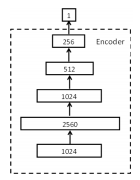
\includegraphics{online.PNG}
    \caption*{Рисунок 1 - Архитектура online-обучения DLT}
\end{figure}

 Отслеживаемый объект указывается расположением его ограничительной рамки в первом кадре. Некоторые негативные примеры собраны из фона на небольшом расстоянии от объекта. Далее сигмоидальный классификационный слой добавляется в часть SDAE, полученную в результате автономного обучения. Общая сетевая архитектура показана на рисунке (1). Когда считывается новый видео-кадр, сначала вычисляются фильтр-частицы в соответствии с подходом, описанным выше. Затем достоверность каждой частицы определяют путем простого прямого прохода через сеть. 
 
 Примечательно то, что вычислительные затраты на этом этапе очень низки, не смотря на высокую точность.

\subsection{Квантование весов}

Известно, что реализация нейронной сети задействует много памяти для хранения, как минимум, матрицы весов для каждого слоя нейронов. Так как мы рассматриваем глубокое обучение, в нашем случае - множество матриц перехода, из-за чего данное хранение является дорогостоящей опцией.

Данную проблему можно решить с помощью использования вместо ячейки памяти - мемристора. Данный подход описан в статье [9]. Нам необходимо после предобучения нашей сети, при запуске частного случая - это после загрузки весов обученной сети, нам необходимо провести квантование данной матрицы. 

Алгоритм квантования матриц весов для алгоритма DLT можно наблюдать в подробнее с помощью кода на Matlab (Приложение).

\subsection{Постановка задачи}

В данном случае общая постановка задачи заключается в определении положения объекта на наборе изображений. Для этого нам необходимо определять центр объекта, его границы, некую рамку в которую помещается объект, на каждом кадре-изображении.

Таким образом необходимо разобраться с алгоритмом определяющим искомый объект в рамку, выявить его слабые стороны, применить алгоритм, модернизирующий данный, и оценить его влияние на исходный алгоритм.

\newpage
\section*{Глава 2. Результаты}
\addcontentsline{toc}{section}{Глава 4. Результаты}

\setcounter{section}{4}
\setcounter{subsection}{0}

\subsection{Реализация}
 Для реализации алгоритма DLT был использован MATLAB версии R2019b 9.7. Язык MATLAB - является высокоуровневым, имеет широкий спектр функций, интегрированную среду разработки, объектно-ориентированные возможности и интерфейсы к программам. Также в нем имеются такие наборы инструментов, как Neural Network Toolbox и различные математические пакеты, удобные для вычисления сложных алгоритмов.
 
 \begin{figure}[h]
    \label{car4}
    \centering
    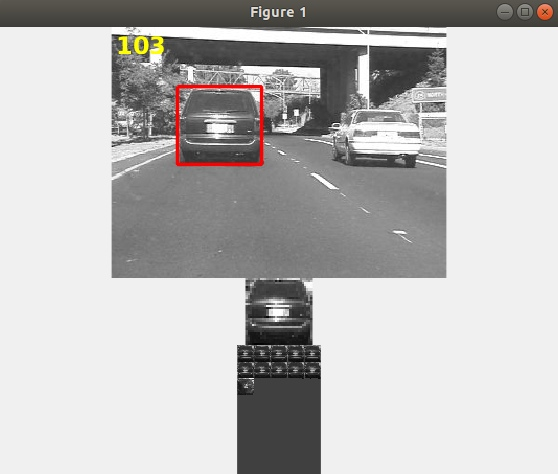
\includegraphics[width=10cm]{CySy3-U4mFg.jpg}
    \caption*{Рисунок 2 - Использование DLT на примере видео car4}
\end{figure}
 
 Также можно наблюдать работу данной программы в режиме реального времени, наблюдая на экране по-кадровый вывод на котором красной рамкой демонстрируется траектория объекта, подсчитанная с помощью алгоритма DLT. На рисунке (2) мы можем наблюдать работу этой программы для конкретной последовательности car4.
 
\subsection{Эксперименты}
\subsubsection{Входные данные}
В качестве входного наборов видео для тестирования моделей, были использованы наборы изображений [3], разработанные специально для тестирования подобных моделей. В данном наборе присутствует $50$ экземпляров видео последовательностей которые можно использовать для тестирования моделей слежения за объектами.

Тестирование проводилось с помощью процессора Intel(R) Pentium(R) CPU 2020M 2.40GHz. Заметим сразу, что вычисления можно ускорить, если вычисления проводить с помощью GPU и MATLAB Parallel Computing Toolbox, как для автономного обучения, так и для online-отслеживания.

\subsubsection{Результаты квантования весов}
Зависимость времени работы программы слежения от числа уровней квантования L:

\begin{table}[h]
\centering
\begin{tabular}{|l|l|l|l|l|l|l|l|}
\hline
L                                 & 2 & 4 & 8 & 16 & 32 & 64 & 128 \\ \hline
Время работы программы            &   &   &   &    &    &    &     \\ \hline
Время квантования матриц          &   &   &   &    &    &    &     \\ \hline
Количество кадров в секунду (fps) &   &   &   &    &    &    &     \\ \hline
\end{tabular}
\end{table}

Зависимость среднего смещения центра рамки захвата (в пикселах) от числа уровней квантования L:

\begin{table}[h]
\centering
\begin{tabular}{|l|l|l|l|l|l|l|l|}
\hline
L                    & 2 & 4 & 8 & 16 & 32 & 64 & 128 \\ \hline
Среднее смещение     &   &   &   &    &    &    &     \\ \hline
\end{tabular}
\end{table}

Для $L = 2, 8, 32, 128$ были сняты смещения центра рамки в зависимости от номера кадра. 

\newpage
\section*{Заключение}
\addcontentsline{toc}{section}{Заключение}
В данной работе описан эффективный алгоритм распознавания траектории движения объекта на видео-последовательности. С его помощью можно осуществлять отслеживание объектов эффективнее, чем, например, с помощью органов зрения. 

Таким образом, были достигнуты следующие результаты:
\begin{itemize}[leftmargin=0em, itemindent=2.5 em,itemsep=1.5 pt,parsep=1.5 pt]
    \item[--] Исследован эффективный алгоритм DLT для работы с отслеживанием траектории движения на видеоматериале
    \item[--] Исследован метод сравнения различных моделей слежения между собой
    \item[--] Изучена реализация данных алгоритмов 
    
\end{itemize}


\newpage 
%вывод списка литературы из библиотеки 
\section*{Список литературы}
\addcontentsline{toc}{section}{Список литературы}
\begin{enumerate}[leftmargin=0em, itemindent=2.5 em,itemsep=1.5 pt,parsep=1.5 pt]
    \item D. Ross J.Lim R. Lin, Yang M. Incremental learning for robust visual tracking -- 2008.
    \item H. Grabner M. Grabner, Bischof H. Real-time tracking via on-line boosting // BMVC -- 2006. -- P.47-56.
    \item Y. Wu, J. Lim and M. Yang, Online Object Tracking: A Benchmark // IEEE Conference on Computer Vision and Pattern Recognition, Portland, OR, -- 2013. -- P. 2411-2418.
    \item Vargas R. Deep Learning: A Review / Mosavi A. Ruiz R. // Advances in Intelligent Systems and Computing. -- 2017.
    \item H. Li C. Shen Q. Shi. Real-time visual tracking using compressive sensing. -- 2011. -- P.1305-1312.
    \item J. Kwon K. M. Lee. Minimum uncertainty gap for robust visual tracking. -- 2013. -- P.2355 -- 2362.
    \item Wang, Naiyan and Yeung, Dit-Yan. Learning a Deep Compact Image
    
    Representation for Visual Tracking // Curran Associates, Inc. -- 2013. -- 809 -- 817.
    \item Guoxing Wu. Regional deep learning model for visual tracking /  Wenjie Lu and Guangwei Gao and Chunxia Zhao and Jiayin Liu. // Neurocomputing -- 2016. -- P. 310 -- 323.
    \item Тарков М.С. Информационная ёмкость сети Хопфилда с квантованными весами // ПДМ -- 2019. -- Р. 97 -- 103.
\end{enumerate}
\newpage
\section*{Приложение}
\addcontentsline{toc}{section}{Приложение}
Реализация квантования матрицы весов:
\begin{verbatim}
 tic;
 quantization_layer = 128; 
    disp(['start quantization L = ' num2str(quantization_layer)]);
    for g = 1 : 4
        w_max_str = max(abs(W{1,g}));
        w_max = max(abs(w_max_str));
        delta = w_max/(quantization_layer - 1);
        colich = newNN.size(g)+1;
        colich_2 = newNN.size(g+1);
        for d = 1 : colich_2
            for e = 1 : colich
                for k = 1 : quantization_layer
                   w = W{1,g}(d,e);
                    if w > (k-1)*delta && w < k*delta
                        W{1,g}(d,e) = (k-1)*delta*sign(w);
                    end
                end
            end
        end
    end
    time = toc;
    disp(['end quantization ' num2str(time)]);
    save(['quant_res_' int2str(quantization_layer)],'W');
\end{verbatim}
\end{document}  % КОНЕЦ ДОКУМЕНТА !